\documentclass [14 pt]{article}
\usepackage[a4paper, total={6in, 8in}]{geometry}

\usepackage{fancyhdr}

\usepackage{hyperref}
\usepackage{graphicx}
\usepackage{float}
\usepackage{color}
\usepackage[english]{babel}
\usepackage[utf8]{inputenc}
\usepackage{listings}
\usepackage{multicol}
\usepackage{subcaption}
\usepackage{caption}
\usepackage{multirow}
\usepackage{titling}
\usepackage{booktabs}
\renewcommand\maketitlehooka{\vfill}
\renewcommand\maketitlehookd{\vfill\null}

\definecolor{deepblue}{rgb}{0,0,0.5}
\definecolor{deepred}{rgb}{0.6,0,0}
\definecolor{deepgreen}{rgb}{0,0.5,0}

\lstset{
language=Python,
	belowcaptionskip=1\baselineskip,
  	frame=single,
  	numbers=left,
  	xleftmargin=\parindent,
  	basicstyle=\ttfamily\scriptsize,
  	showspaces=false,
  	showtabs=false,
 	breaklines=true,
  	showstringspaces=false,
  	breakatwhitespace=false,
    keywordstyle=\color{deepblue},
    stringstyle=\color{deepgreen},
    rulecolor= \color{black},
}

\linespread{1.25}

\title{Project 2: Multi-source code search}
\author{Ardig\`o Susanna}
\date{15 December, 2020}
\begin{document}

\pagestyle{fancy}
\fancyhf{}
\lhead{Ardig\`o Susanna}
\rhead{Knowledge Analysis \& Management}
\cfoot{\thepage}

\begin{titlingpage}
\maketitle
\centering
\url{https://github.com/SusyPinkBash/multi_source_code_search}
\end{titlingpage}

\newpage\thispagestyle{plain}
\tableofcontents
\newpage

\section{Data Extraction} % 1:
\subsection{Goal and Input parameter} % 1: goal & input
This part of the project consists of extracting names and comments of Python classes, methods and functions and save them in a csv file.\\
This file takes as argument the path of the directory of the project that we want to analyze. For this project we use the project \texttt{tensorflow}.

\subsection{Description of the code} % 1: code description
To efficiently parse the files in the directory, we created a class named \texttt{Visitor}, which extends the \href{https://docs.python.org/3/library/ast.html#ast.NodeVisitor}{\texttt{NodeVisitor}} class of the standard library ast (which stands for Abstract Syntax Tree). This class holds the path of the file. There is a global variable \texttt{data} used throughout the execution to store all the information extracted.\\
The function \texttt{start(directory\_path)} \emph{`walks'} the given directory using the function \texttt{walk} which generates a 3-tuple of directory path, directory names and file names. We open and read all the python files, checked with the extension of the file, we create a Visitor object and start to visit. The class we created has two different visit methods which differ in if the node visiting is a definition of a class or a function.
The method \texttt{visit\_FunctionDef(self, node: FunctionDef)} adds the node information to the array of data if the function or method is not a main or a test. Since this method is used both for functions and methods, we know if the node is a method by checking if the first argument is \texttt{self}.
The method \texttt{visit\_ClassDef(self, node: ClassDef)} calls a generic visit (of the ast library) and, as the previous method, adds the node information to the array of data if the class is not a main or a test. \\
After the parsing is complete we create a pandas dataframe, feeding it as data the data array, and export it in a csv extension.

\subsection{Results}
% 1: results
Table \ref{tab:DataExtraction} show the number of Python files, classes, methods and functions found while parsing the Tensorflow directory. The results can be found in the file \texttt{res/data.csv}.

\begin{table}[h]
\centering
\begin{tabular}{| l r |}
\hline
\textbf{Type}	&  \textbf{\#}	\\ \hline\hline
Python files 	&	2817	\\
Classes			&	1904	\\
Methods			&	7271	\\
Functions		&	4881	\\ \hline
\end{tabular}
\captionof{table}{Count of data found in Tensorflow}\label{tab:DataExtraction}
\end{table}

\section{Training of search engines} % 2
\subsection{Goal and Input parameter} % 2: goal & input
This part of the project consists of representing code entities using the four embeddings frequency, TF-IDF, LSI and Doc2Vec.\\
This file takes as argument a query which will be fed to the four search engines. 

\subsection{Description of the code} % 2: code description
The function \texttt{start(query)} loads the csv into a pandas dataframe and then computes the results.
The first part of function \texttt{compute\_results(query, dataframe)} creates the necessary data and normalizes the query that the second part needs to produce the results.\\
The first part of function \texttt{create\_data(dataframe)} extracts the names and comments of the data extracted in the first part. to create a clean array of arrays of tokens and a dictionary with the frequencies of each token. In the second part we create the corpus by processing the tokens, we create a gensim dictionary and the bag of words. At the end of the creation, we save the corpus, dictionary and bag of words in external files to then load them in future runs.
In the second part of function \texttt{compute\_results(query, dataframe)} we create a dictionary that hold the results of the searches and a dictionary to save the embedding vectors. \\
The function \texttt{query\_frequency(query, bow, dictionary)} creates a sparse matrix of the bag of words and returns an array with the similarity scores of each entity of the given csv file. This array is then filtered to extract only the top 5 scoring entities.
Similarly, the function \texttt{query\_tfidf(query, bow, dictionary)} creates a sparse matrix of the tfidf model of the bag of words and returns an array with the similarity scores which is then filtered.
The function \texttt{query\_lsi(query, bow, dictionary)} creates a lsi model based on the bag of words, a vector based on the model and the dictionary, the matrix of the similarities and the embedding vectors. The result of the matrix, as in the previous cases, is filtered to get only the top 5 scores.
The function \texttt{query\_doc2vec(query, bow, dictionary)} creates a doc2vec model which then feed the corpus to and train it. We create a vector infering it from the query, we create the similarity and take only the top 5 scores and the embedding vectors.\\
We save the trained models in external pickle files to load then load them in the next runs. This improves the running time of the function.\\
We create a dataframe with the information stored in the dictionary, we print the results and save them in a separate file.

\subsection{Results} % 2: results
To show the results we run this part of the project with the query:\\
\centerline{\emph{`AST Visitor that looks for specific API usage without editing anything'}}.\\
% 2 : comment results 
The correct document is \texttt{PastaAnalyzeVisitor} with path \texttt{../tensorflow/tensorflow/tools/\\compatibility/ast\_edits.py}.\\
Figure \ref{fig:Part2} show the result of the given query.\\
As we can see in the image all search engine find the correct document as a first result. 
We can see that Frequency and TF-IDF have three results in common, if we don't consider the correct result, but at different positions. 
\begin{figure}[h]
\centering
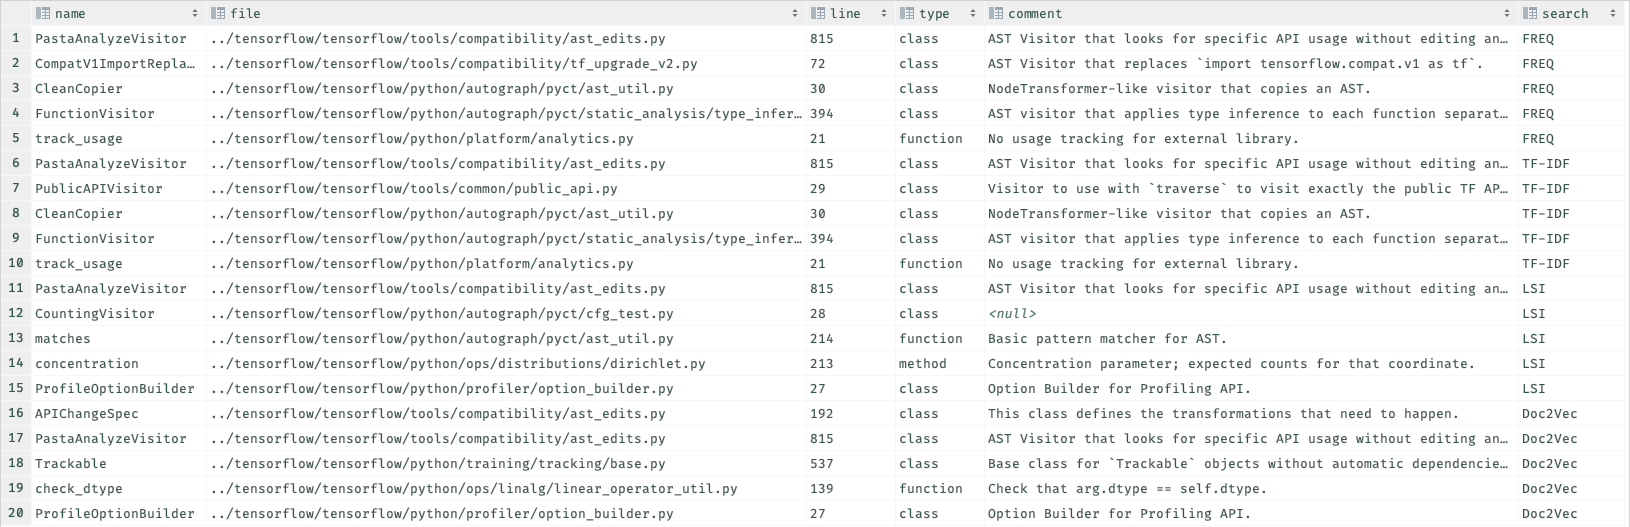
\includegraphics[width=0.95\textwidth]{../res/part2.png}
\caption{Results of the given query}\label{fig:Part2}
\end{figure}


\section{Evaluation of search engines} % 3
\subsection{Goal and Input parameter} % 3: goal & input
This part of the project consists of measuring the precision and recall given 10 queries along with their ground truth.\\
This file takes as argument the path of the ground truth file.

\subsection{Description of the code} % 3: code description
The function \texttt{start(path\_ground\_truth)} loads the csv of the data  into a pandas dataframe, parses the ground truth and then computes the precision and recall.\\
To efficiently parse the ground truth file, we created a class named \texttt{Truth} which holds the name, path and query. We read the ground truth file and create an array with all the entries of the ground truth and the queries.\\
To compute precision and recall we get the data of the results and the embedding vectors from the previous part. We create a dictionary to save the scores of the queries and a dictionary for the vectors. We then compute the precision and recall, by comparing our results and the ground truth.

\subsection{Results} % 3: comment results
Table \ref{tab:Evaluation} show the statistics of precision and recall compared to the unique ground truth.
We can see that the precision is high for all engines except for one. The engine with the highest precision is \texttt{TF-IDF}, with score 8.85.
The second highest precision is \texttt{Frequencies}, with score 0.83.
The third highest precision is \texttt{LSI}, with score 0.80.
The least precise search engine is \texttt{Doc2Vec} with score 0.55, which is the only score lower than $0.8$\\
The recall is higher than the precision. The \texttt{TF-IDF} engine has a recall equal to $1$, which means that for each query the search engine has found the correct result in the top 5. The second highest recall is of \texttt{Frequencies} with score $0.9$. It is followed by \texttt{LSI} with a score of $0.9$. At last \texttt{Doc2Vec} has a recall of $0.6$.\\
We can say that almost all search engine have similar scores for precision and recalls. The only exception is \texttt{Doc2Vec}.\\

\begin{table}[h]
\centering
\begin{tabular}{| l r r |}
\hline
\textbf{Engine}	&  \textbf{Precision}	&  \textbf{Recall}	\\ \hline\hline
Frequencies 		&	0.83	&	0.90	\\
TD-IDF			&	0.85	&	1.00	\\
LSI				&	0.80	&	0.80	\\
Doc2Vec			&	0.55	&	0.60	\\ \hline
\end{tabular}
\captionof{table}{Statistics of the search engines}\label{tab:Evaluation}
\end{table}


\section{Visualisation of query results} % 4
\subsection{Goal and Input parameter} % 4: goal & input
This part of the project consists of visualizing the embedding vectors of the queries and the top 5 answers in a 2D plot.
This file takes as argument the ground truth file.

\subsection{Description of the code} % 4: code description
The first part of the execution is the same as the previous file. After the results are calculated, we use the embedding vectors, that we retrieved in the explanation above but we did not use. For vector we apply TSNE to produce 2D vectors composed of queries and the top 4 results.
The plot is straight-forward: we create a dataframe with the information of x and y coordinates and print them of different hues. We use the library \texttt{seaborn} to create the charts and we then save them on disk.

\subsection{Results} % 4: comment results
Figures \ref{fig:lsi} and \ref{fig:doc2vec} shows the plots of the visualization of the queries. At first we notice that the LSI scatterplot tends to have better query clusters. The optimal solution is to have defined clusters for each query. This does not happen in any of the two images. There are queries that create clusters but this does not happen for all queries.\\

\subsubsection{LSI}
\begin{figure}[H]
\centering
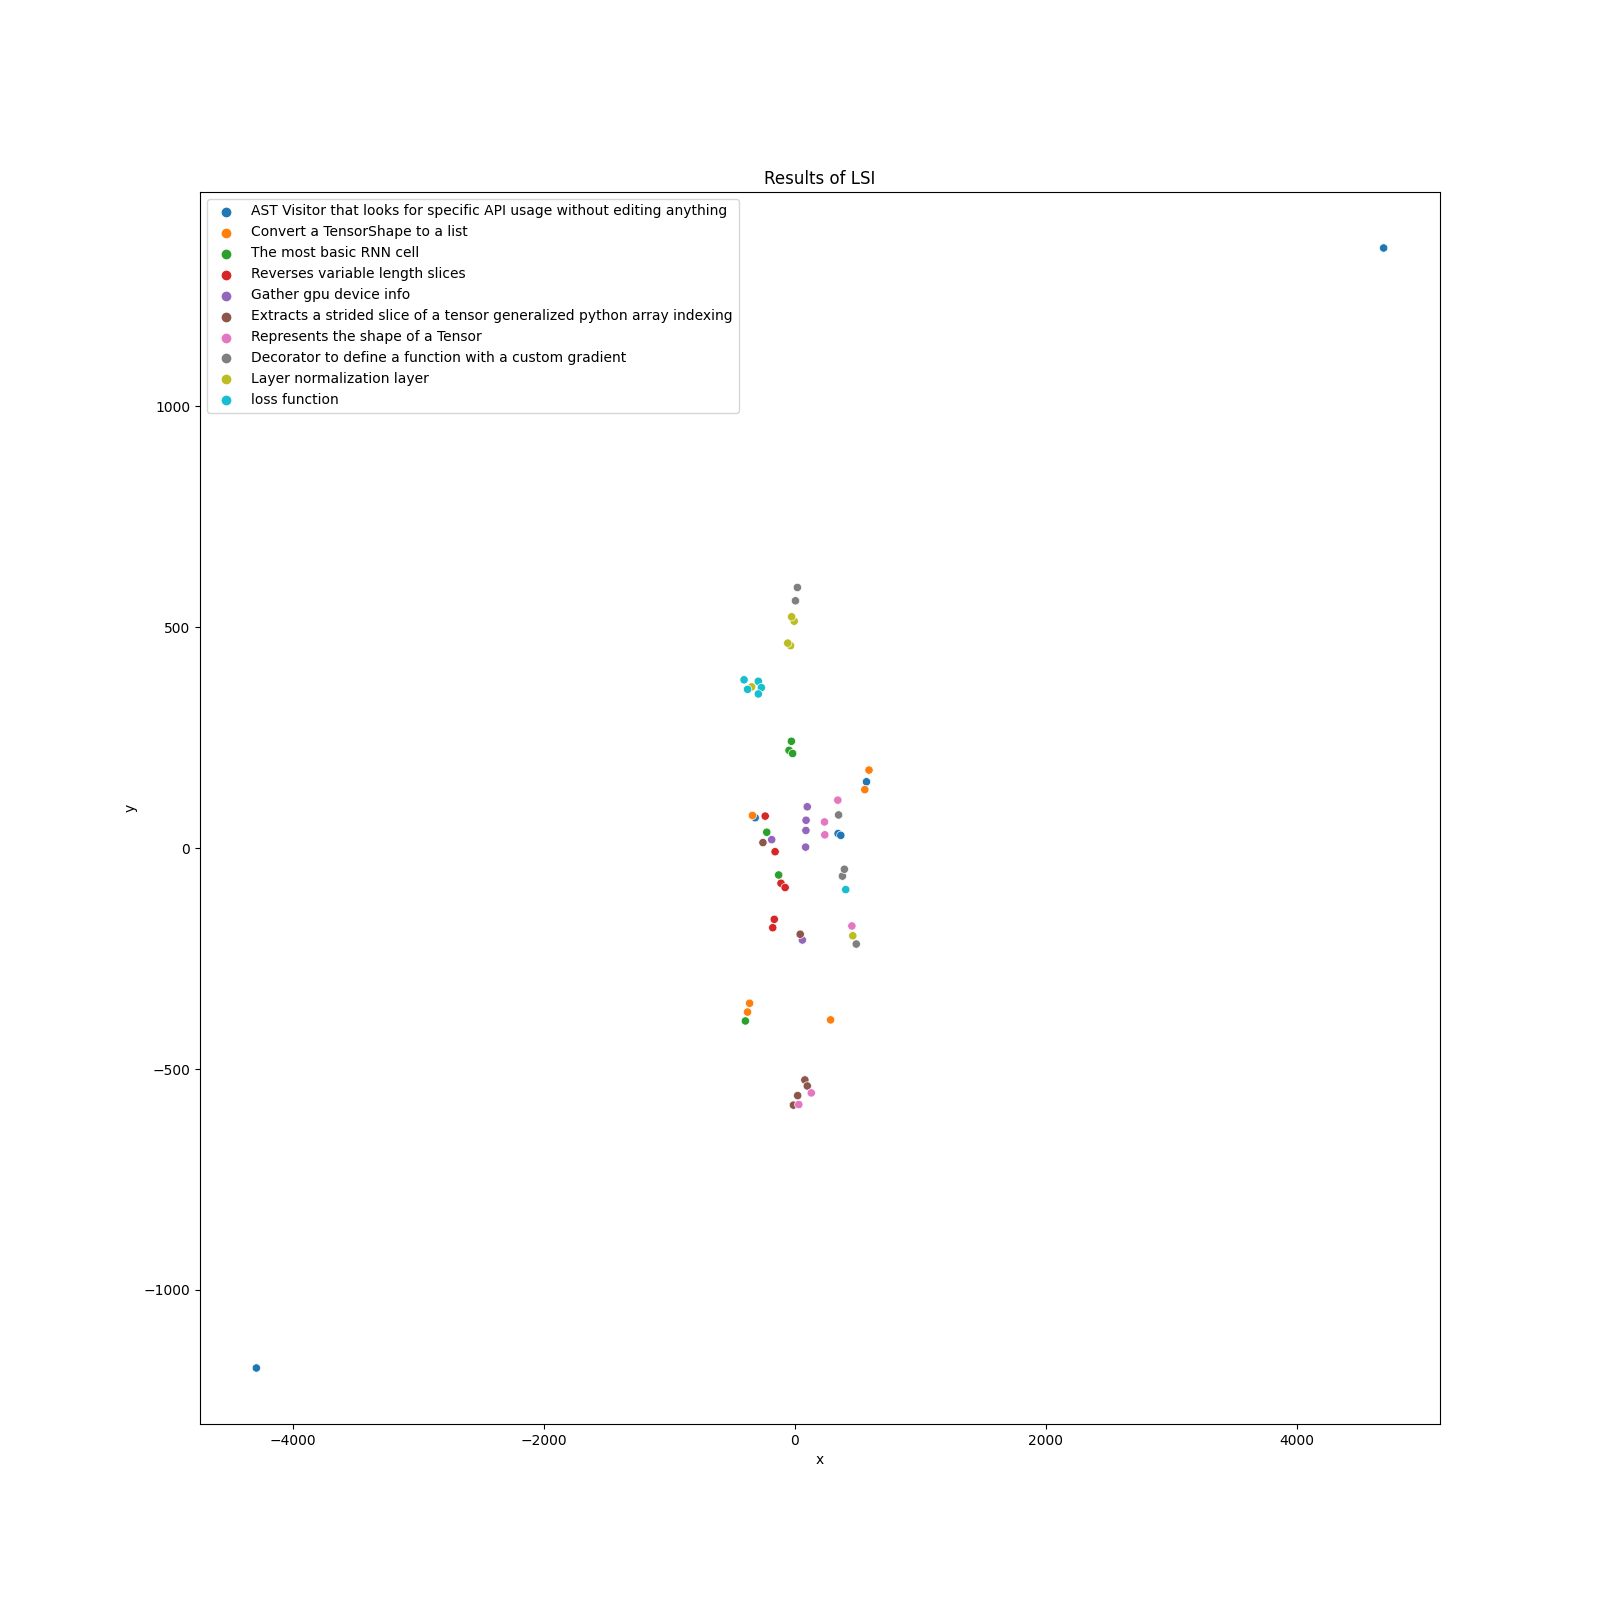
\includegraphics[width=0.84\textwidth]{../res/lsi.png}
\caption{Visualization of the queries using LSI}\label{fig:lsi}
\end{figure}
Analyzing the plot of LSI, shown in figure \ref{fig:lsi}, we can see that some results of the queries tend to stay close, but not completely. There are some well defined clusters composed of the same queries. Some examples are \emph{loss function}, \emph{The most basic RNN cell} and \emph{Reverses variable length slices}. 
The queries of \emph{Convert a TensorShape to a list} and \emph{Decorator to define a function with a custom gradient} that tend to have some results that are somewhat close.


\subsubsection{Doc2Vec}
\begin{figure}[H]
\centering
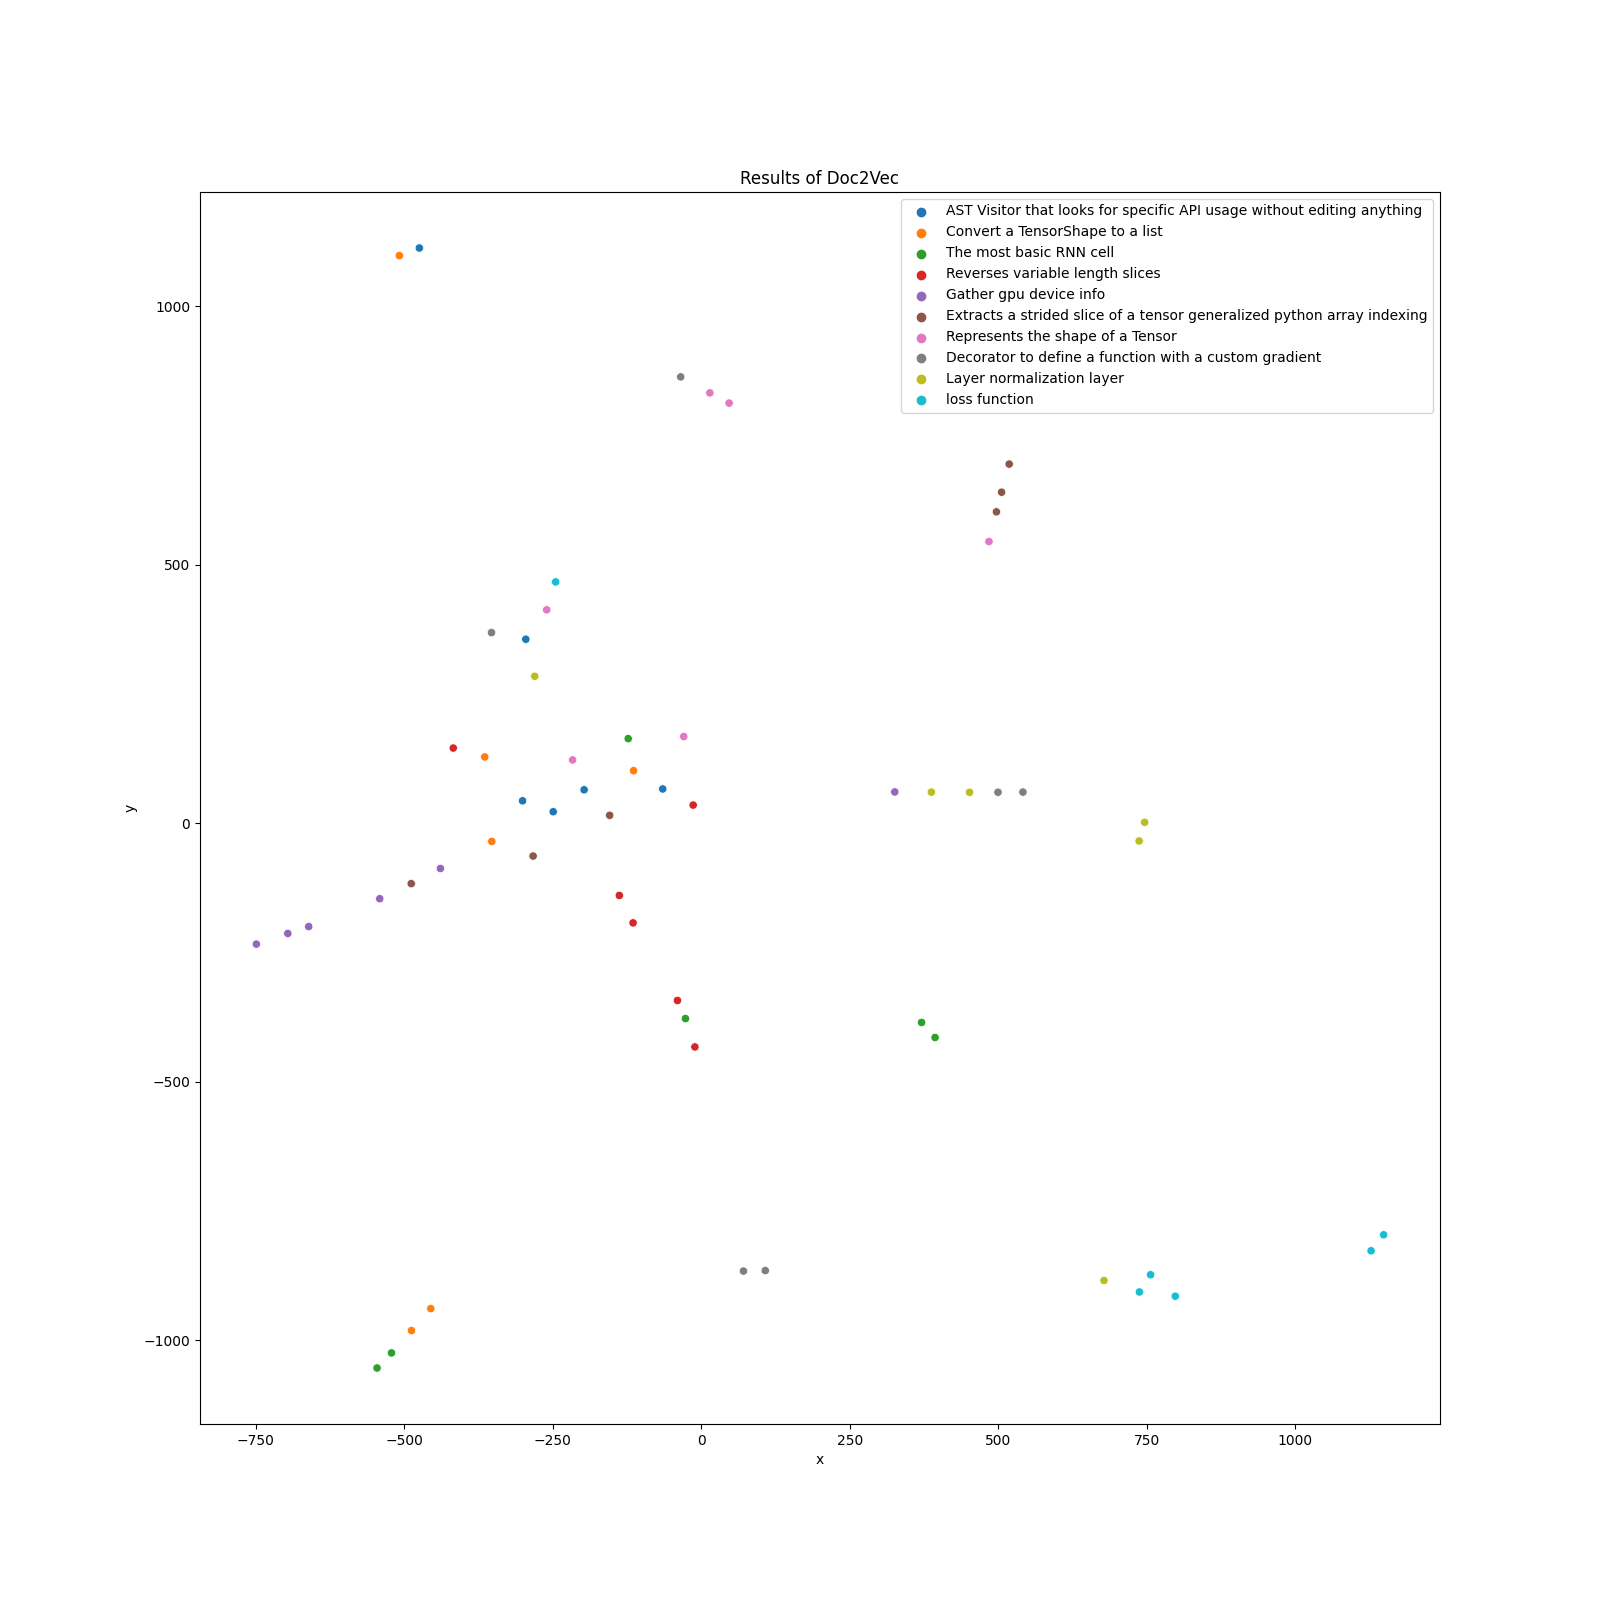
\includegraphics[width=0.84\textwidth]{../res/doc2vec.png}
\caption{Visualization of the queries using Doc2Vec}\label{fig:doc2vec}
\end{figure}
Analyzing the plot of Doc2Vec, shown in figure \ref{fig:doc2vec}, we can see that there are  results of the queries tend to stay closer than the previous plot.
In this image there are some cluster that are well defined and are composed only of one query. Some queries are divided into two clusters close to each other.
The most well defined cluster is \emph{`loss function'}, which was also well defined in the previous plot. 
There is a cluster which is composed of five different queries.


%\begin{figure}[h]
%\centering
%\begin{subfigure}[t]{0.4\textwidth}
%\centering
%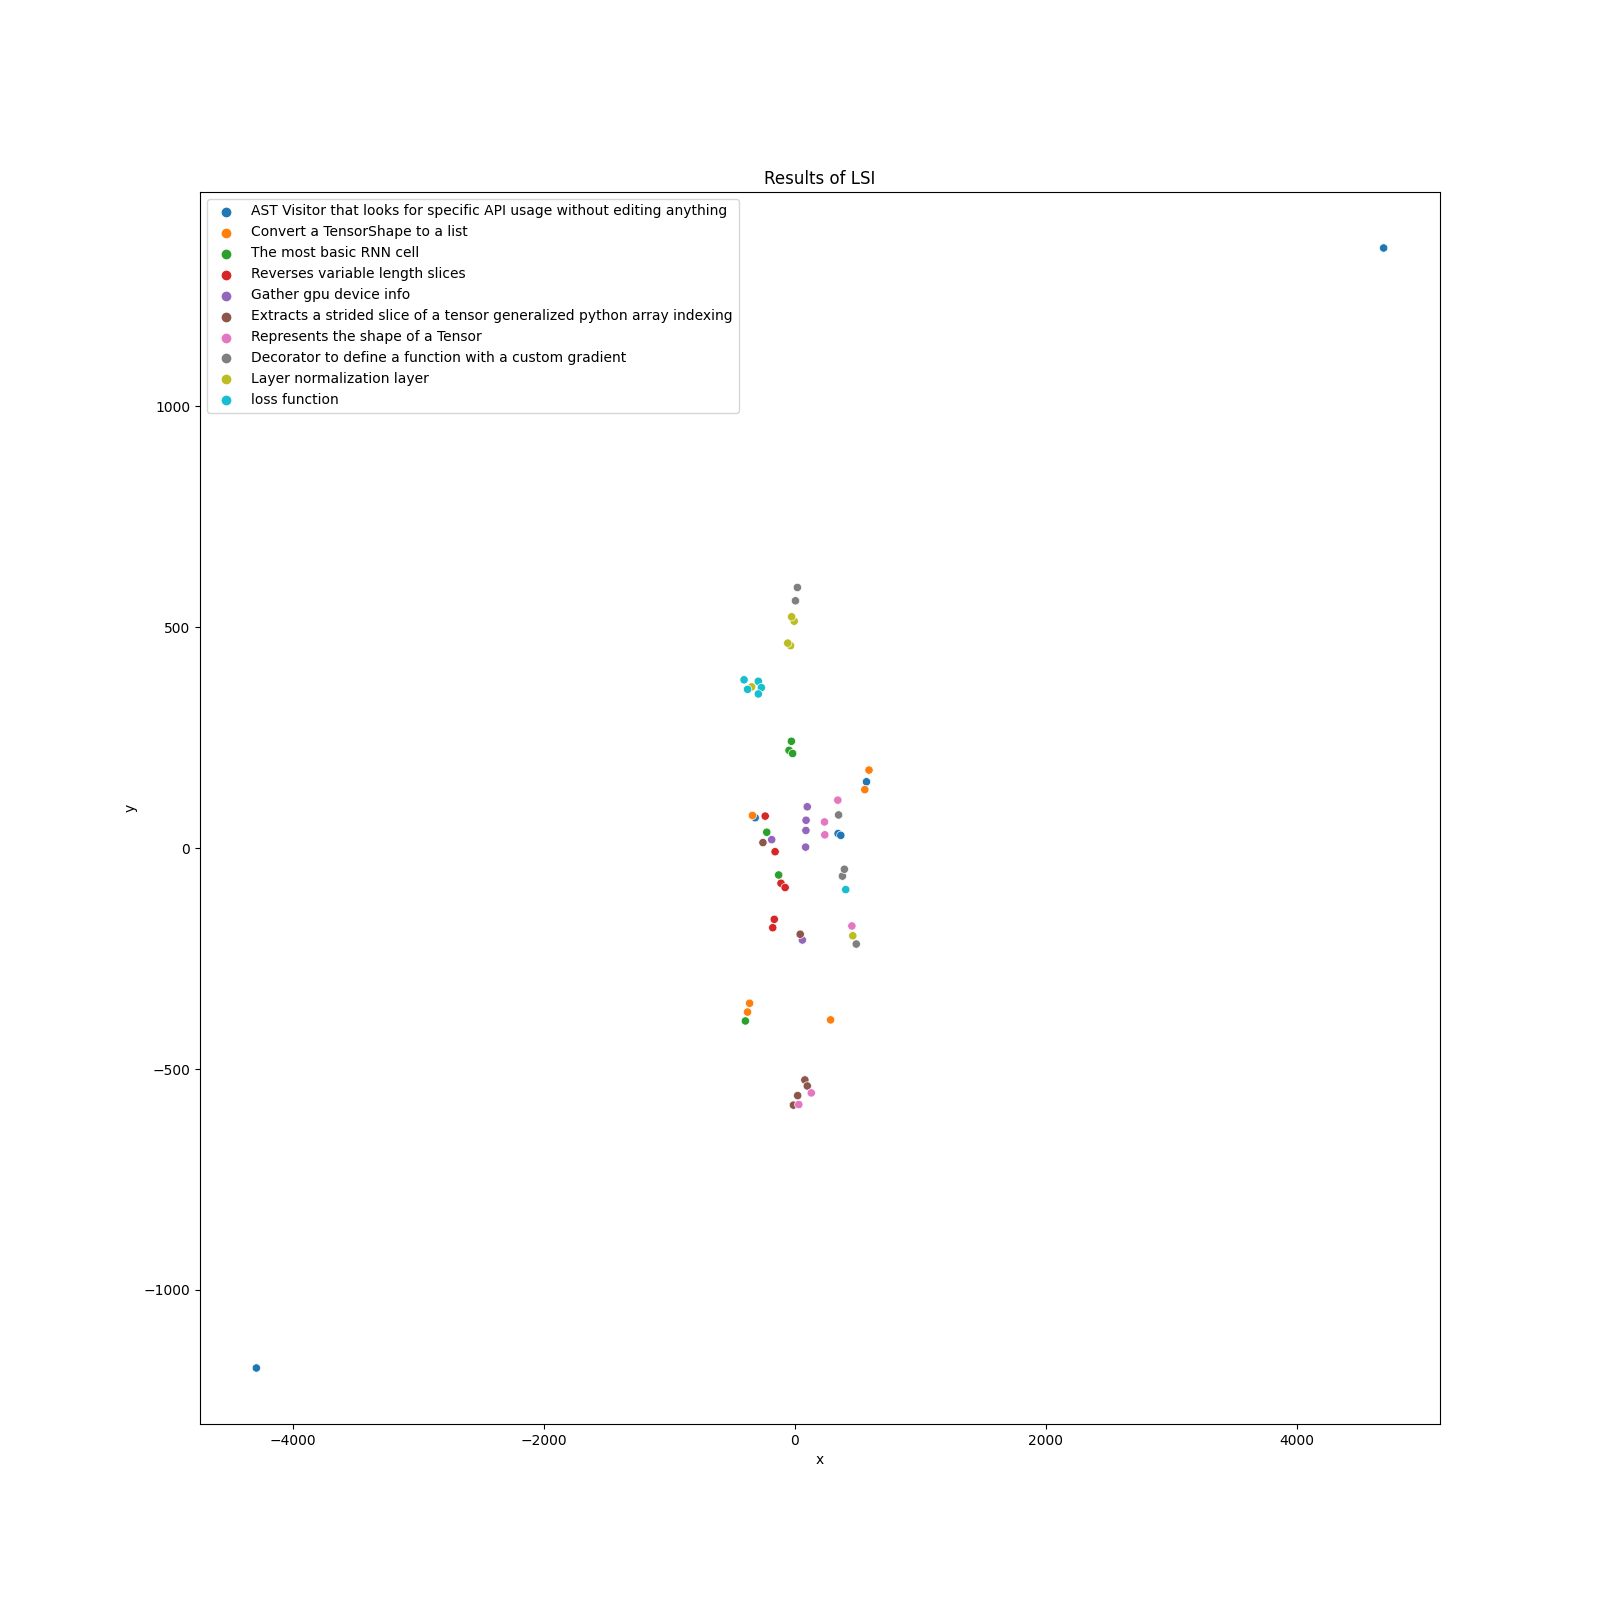
\includegraphics[width=\textwidth]{../res/lsi.png}
%\caption{Results of LSI}\label{fig:lsi}
%\end{subfigure}
%\hfil
%\begin{subfigure}[t]{0.4\textwidth}
%\centering
%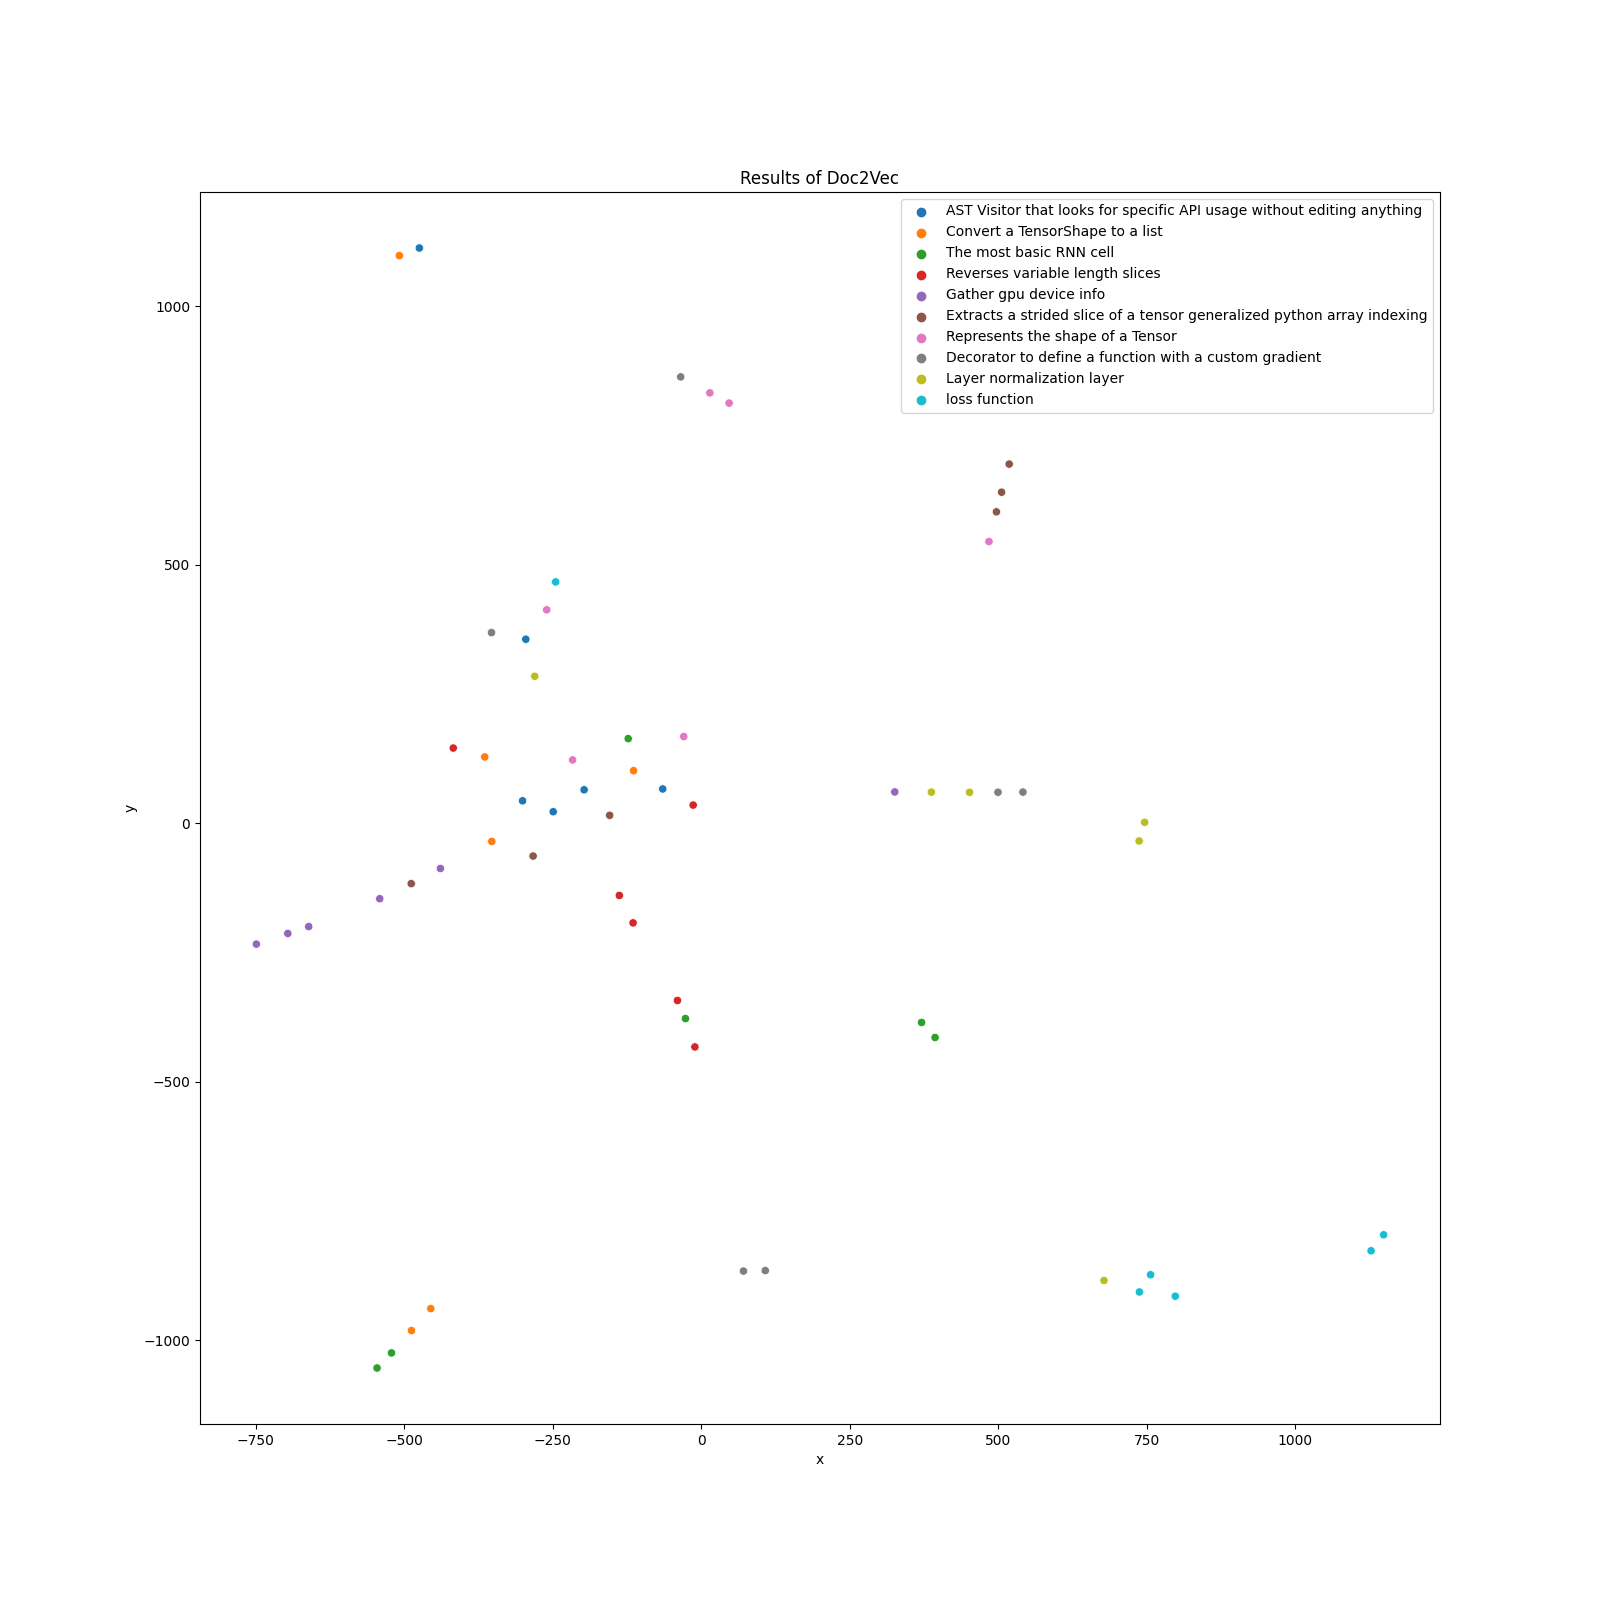
\includegraphics[width=\textwidth]{../res/doc2vec.png}
%\caption{Results of Doc2Vec}\label{fig:doc2vec}
%\end{subfigure}
%\caption{Visualization of the plots of the queries}
%\label{fig:plots}
%\end{figure}

\newpage
\appendix

\section{Python code}

\subsection{Data Extraction}
\lstinputlisting{../src/extract_data.py}
\subsection{Training of search engines}
\lstinputlisting{../src/search_data.py}
\subsection{Evaluation of search engines and Visualisation of query results}
\lstinputlisting{../src/prec_recall.py}
\newpage

\section{Bash Code} 
\lstinputlisting[language=Bash]{../run.sh}

\end{document}